\documentclass[10pt]{article}

% --- Page Setup ---
% \usepackage[a4paper, margin=0.5cm]{geometry}
\usepackage[a4paper, left=0.5cm, right=0.5cm, top=0.3cm, bottom=0.3cm]{geometry}
\usepackage{multicol}

% \allowdisplaybreaks

\usepackage{booktabs} % Required for professional horizontal rules (\toprule, \midrule, \bottomrule)
\usepackage{array}    % Required for better column formatting

% --- Math and Code ---
\usepackage{amsmath, amssymb}
\usepackage{listings}

% --- Spacing Adjustments ---
\usepackage{enumitem}
\usepackage{titlesec}

\usepackage{nicematrix, tikz}

\usepackage{graphicx}

\usepackage{float}

\usepackage[hidelinks]{hyperref} % hidelinks removes ugly red boxes around links

% 1. Remove space between list items
\setlist{nosep, leftmargin=*} 

% 2. Shrink space around section headers
\titlespacing*{\section}{0pt}{0pt}{0pt}
\titlespacing*{\subsection}{0pt}{1ex plus .2ex minus .2ex}{0.5ex plus .1ex}

% --- NEW: Reduce header font sizes ---
\titleformat*{\section}{\normalsize\bfseries\color{blue!75!black}}
\titleformat*{\subsection}{\small\bfseries\color{magenta}}

% 3. Add a thin line between columns for readability
\setlength{\columnseprule}{0.4pt}
\setlength{\columnsep}{1.5em}

% --- Custom Code Formatting ---
\lstset{
    basicstyle=\ttfamily\scriptsize,
    breaklines=true,
    aboveskip=2pt,
    belowskip=2pt
}

\usepackage{xcolor}
% \newcommand{\sectionbox}[1]{%
%      \colorbox{blue!75!black}{\color{white}\small\bfseries~#1~}%
%    }
%    \titleformat{\section}{}{}{0em}{\sectionbox}
%    \titleformat*{\subsection}{\normalsize\bfseries}

\raggedbottom

\setlength{\parskip}{0pt}
\setlength{\baselineskip}{0pt plus 0.2pt} 

\begin{document}

% ==== from cheatsheet2.tex ====
\small 

\raggedright

\tableofcontents

\newpage

\begin{table}[H]
    \centering
    \footnotesize % Reduces font size for cheatsheet
    \renewcommand{\arraystretch}{1.2} % Tighter row spacing
    \begin{tabular}{@{} l p{2.2cm} l p{4.5cm} p{3.5cm} @{}}
        \toprule
        \textbf{Memory} & \textbf{Layout \& Cost} & \textbf{Speed} & \textbf{Implementation Insights} & \textbf{Transistor Function} \\
        \midrule
        \textbf{SRAM} & 
        Larger (6T) \newline High Cost & 
        Very Fast & 
        \textbf{CPU Cache:} Demands raw speed. Small capacity (KB/MB) justifies cost. High R/W endurance. & 
        Store data \& control signal transfer. \\
        
        \textbf{DRAM} & 
        Smaller (1T, 1C) \newline Low Cost & 
        Slower \newline (Refresh) & 
        \textbf{System RAM:} OS/Apps need massive capacity (GBs); SRAM is too expensive. Handles heavy R/W cycles. & 
        Access switch to charge/discharge data capacitor. \\
        \bottomrule
    \end{tabular}
    \caption{Volatile Memory Summary}
\end{table}

\begin{table}[H]
    \centering
    \footnotesize 
    \renewcommand{\arraystretch}{1.2} 
    \begin{tabular}{@{} l p{2.8cm} p{1.8cm} p{3cm} p{3.8cm} @{}}
        \toprule
        \textbf{Memory} & \textbf{Layout \& Arch.} & \textbf{Cost / Cap.} & \textbf{Erasure / Granularity} & \textbf{Implementation Insights} \\
        \midrule
        \textbf{EPROM} & 
        \textbf{1T}. Needs quartz window for UV. & 
        High \newline Low Cap. & 
        Very Slow ($\sim$15m) \newline Full Chip Erase & 
        Legacy storage; rarely used today. \\
        
        \textbf{EEPROM} & 
        \textbf{2T} (Storage + Access). Large footprint. & 
        Very High \newline Very Low & 
        Slow ($\sim$5ms/byte) \newline Byte-level erase & 
        \textbf{Micro-storage:} Saves small system variables. 2T isolates bytes. \\
        
        \textbf{NOR Flash} & 
        \textbf{1T}. \textbf{Parallel} wiring. Dedicated buses. & 
        Medium \newline Medium Cap. & 
        Moderate ($\sim$1s/blk) \newline Block Erase & 
        \textbf{Boot Memory:} Parallel wiring allows random access \& XIP. \\
        
        \textbf{NAND Flash} & 
        \textbf{1T}. \textbf{Series} strings. Multiplexed I/O. & 
        Very Low \newline Very High & 
        Fast ($\sim$1.5ms/blk) \newline Page write, Block erase & 
        \textbf{SSDs/Storage:} Series wiring maximizes density. No XIP. \\
        \bottomrule
    \end{tabular}
    \caption{Non-Volatile Memory Summary}
\end{table}

\begin{table}[H]
    \centering
    \footnotesize 
    \renewcommand{\arraystretch}{1.2} 
    \begin{tabular}{@{} l p{2.5cm} p{1.8cm} p{2cm} p{3.2cm} p{2cm} @{}}
        \toprule
        \textbf{Mechanism} & \textbf{Controller / Nature} & \textbf{Latency} & \textbf{CPU Eff.} & \textbf{Transfer Rate / Modes} & \textbf{Debugging} \\
        \midrule
        \textbf{Polling} & 
        \textbf{CPU} \newline SW-driven active check. & 
        \textbf{Very Fast} \newline 1--3 cycles. & 
        \textbf{Very Low} \newline 100\% blocked. & 
        \textbf{Low} \newline CPU fetches per byte. & 
        \textbf{Easy} \newline Deterministic. \\
        
        \textbf{Interrupt} & 
        \textbf{CPU} \newline HW trigger, SW exec. & 
        \textbf{Slower} \newline Context switch. & 
        \textbf{High} \newline Free until signaled. & 
        \textbf{Moderate} \newline CPU still moves data. & 
        \textbf{Difficult} \newline Asynchronous. \\
        
        \textbf{DMA} & 
        \textbf{DMAC} \newline Pure HW controller. & 
        \textbf{Moderate} \newline Bus arbitration. & 
        \textbf{Very High} \newline CPU fully freed. & 
        \textbf{Maximum} \newline Burst, Steal, Transparent. & 
        \textbf{Moderate} \newline Silent RAM alters. \\
        \bottomrule
    \end{tabular}
    \caption{I/O Data Transfer Mechanisms Summary}
\end{table}

\begin{table}[H]
    \centering
    \footnotesize 
    \renewcommand{\arraystretch}{1.2} 
    \begin{tabular}{@{} l p{3.5cm} p{3.5cm} p{4.5cm} @{}}
        \toprule
        \textbf{Feature} & \textbf{Solid-State Drive (SSD)} & \textbf{Hard Disk Drive (HDD)} & \textbf{Implementation Insights} \\
        \midrule
        \textbf{Mechanics \& Weight} & 
        \textbf{Lighter}, with less/no moving parts. & 
        Heavier, relies on mechanical spinning platters and read/write heads. & 
        \textbf{SSD Advantage:} Highly resistant to physical shock and ideal for portable electronics (laptops/phones). \\
        
        \textbf{Transfer Rate} & 
        \textbf{Higher} (purely electronic memory access). & 
        Lower (bottlenecked by mechanical seek time and disk RPM). & 
        \textbf{SSD Advantage:} Drastically faster OS boot times and application loading. \\
        
        \textbf{Cost per Bit} & 
        Higher. & 
        \textbf{Lower}. & 
        \textbf{HDD Advantage:} The most cost-effective solution for massive, terabyte-scale bulk storage and backups. \\
        
        \textbf{Erase Cycles} & 
        \textbf{Finite} (Flash memory cells physically degrade with repeated writes). & 
        \textbf{Infinite} (Magnetic polarity can be flipped endlessly without wear). & 
        \textbf{HDD Advantage:} Superior for systems that require constant, heavy, 24/7 data rewriting (e.g., security camera DVRs). \\
        \bottomrule
    \end{tabular}
    \caption{Storage Architecture Comparison: SSD vs. HDD}
\end{table}

\newpage

\begin{multicols}{2}

\section*{Computer Arithmetic}
\phantomsection
\addcontentsline{toc}{section}{Computer Arithmetic}
Carry = 1 if '1' bit gets carried out of MSB. Indicates error in unsigned no. system.\\
V = 1 if 
\begin{itemize}
    \item \textbf{A+B}, MSB(A) = MSB(B) $\neq$ MSB(Result)
    \item \textbf{A-B}, MSB(A) $\neq$ MSB(B) and MSB(Result) $\neq$ MSB(A)
\end{itemize}
\textbf{Sign extension}: copy MSB to all the higher bits.\\
\textbf{Multi-precision arithmetic}: add the lower 32-bit words, then ADC the upper 32-bit words.\\
\textbf{Range of 2's comp} = $-2^{N-1}$ to $2^{N-1}-1$\\
\textbf{Fixed point}
\begin{itemize}
    \item Precision = value of LSB (smallest fractional value)
    \item $2^3\,2^2\,2^1\,2^0\,.\,2^{-1}\,2^{-2}\,2^{-3}\,2^{-4}$, precision is $2^{-4}$.
    \item Precision is fixed and uniform throughout the range.
    \item For a fixed number of bits, allocating more bits for the integer part (increase range) will reduce the precision.
\end{itemize}
\textbf{Floating point}
\begin{itemize}
    \item 32-bit: 1 (Sign), 8 (exponent, $E$), 23 (fraction, $F$), bias = 127
    \item 64-bit: 1 (Sign), 11 (exponent, $E$), 52 (fraction, $F$), bias = 1023
    \item Format: $(-1)^S \times (1.F)_2 \times 2^{E - \text{Bias}}$
    \item E.g. 1 00001100 010100....0 $\equiv$ $-1.3125\times 2^{-115}$
    \item Normalised mode
    \begin{itemize}
        \item Maintain a non-zero digit (1) before the radix point.
        \item Exponent range: 0000 0001 to 1111 1110
        \item Smallest magnitude: X 0000 0001 0000....0 $\equiv$ $1 \times 2^{-126}$
        \item Largest magnitude: X 1111 1110 1111 ....1 $\equiv$ $\approx 2 \times 2^{127} = 2^{128}$
        \item Underflow: numbers between $-2^{126}$ to $2^{126}$, i.e. values close to zero that cannot be represented.
    \end{itemize}
\end{itemize}
\textbf{Fixed vs floating pt (32-bit)}
\begin{itemize}
    \item Max range (fixed) = $2^{32}$ (no fractional part)
    \item Max range (floating) = $2*2^{128}$ ($-2^{128}$ to $\sim 2^{128}$)
    \item Max precision (fixed) = $2^{-32}$ (no integer part)
    \item Max precision (floating, near to 0) = less than $2^{-126}$
    \item Floating point has higher range and better precision at small numbers, but very coarse precision at the 2 ends of the range. Floating point provides uniform precision across entire range.
\end{itemize}
\textbf{More stuff}
\begin{itemize}
    \item Arithmetic between numbers with huge diff in magnitude: add/subtract numbers of similar smaller magnitude first, to allow their magnitude to be closer to the bigger magnitudes.
    \item To preserve precision AMAP, do division last, as division truncates LSB and loses bits.
\end{itemize}

\section*{Interfaces}
\phantomsection
\addcontentsline{toc}{section}{Interfaces}
Analog signal is continuous (real world), digital is discrete (for processing).\\
\begin{itemize}
    \item Analog signal is equivalent to a digital signal with infinitely small sampling interval.\\
    \item Nyquist Theorem: For digital signal to be able to represent its analog equiv adequately, minimum sampling rate is 2x the freq of analog signal
\end{itemize}
% Analog-to-digital (ADC) \& Digital-to-analog (DAC) convert the signals for processing.
Sequence of processing real-world data:
\begin{itemize}
    \item ADC $\to$ Digital Processor $\to$ DAC $\to$ smoothing filter.
\end{itemize}
\begin{center}
    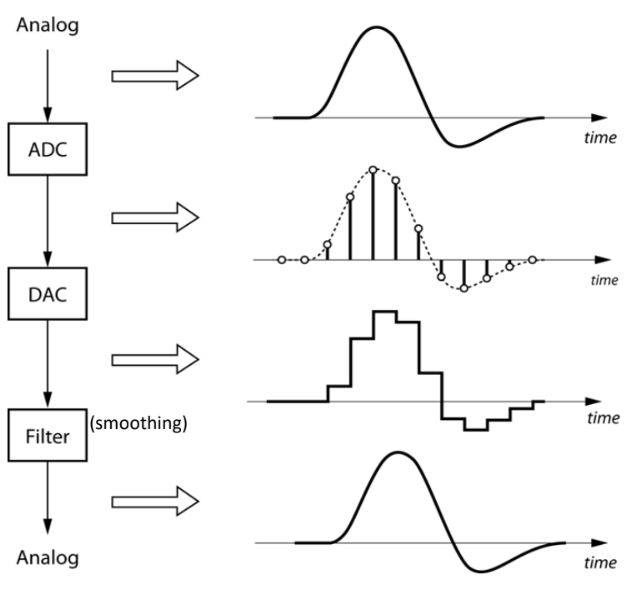
\includegraphics[width=0.3\textwidth]{images/adc-dac.png}
\end{center}
Interface is a boundary where 2 or more devices meet to exchange info.\\
Considerations when interfacing devices:
\begin{itemize}
    \item Electrical signal level: output voltage level should not exceed the max allowable input voltage of the input.
    \item Check compatibility: $V_{OH} > V_{IH}$ and $V_{OL} < V_{IL}$.
\end{itemize}
Signals transmitted by differential signals have better noise tolerance.
\begin{center}
    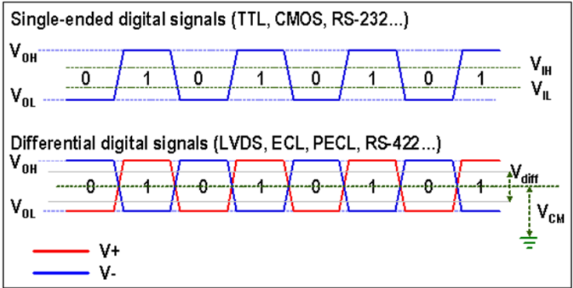
\includegraphics[width=0.35\textwidth]{images/single-vs-differential.png}
\end{center}
\begin{center}
    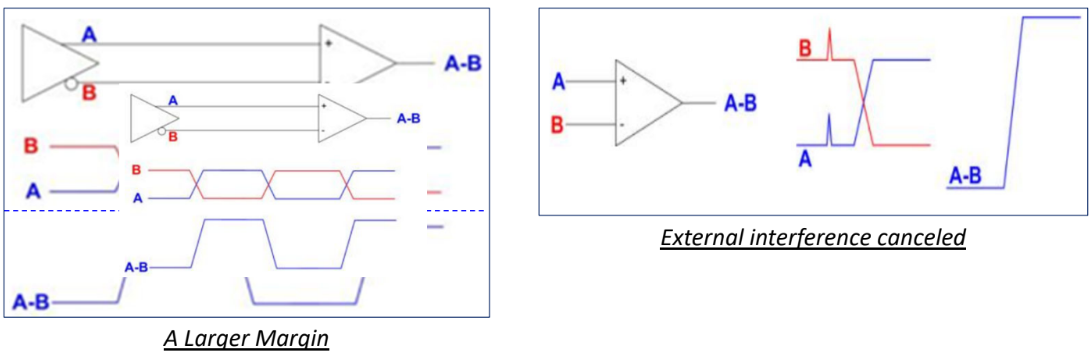
\includegraphics[width=0.4\textwidth]{images/differential-signal.png}
\end{center}
% \textbf{\textcolor{magenta}{Parallel data trf}}\\
\subsection*{Parallel data trf}
\phantomsection
\addcontentsline{toc}{subsection}{Parallel data transfer}
SRAM, DRAM, ROM uses parallel data trf. 
Synchronous in nature with some strobe signal to inform receiver when to latch in the data.\\
Problems:
\begin{itemize}
    \item Signal skew: Signals arrive at diff times 
    \begin{itemize}
        \item Because of variation in propagation delay between signals from the same data bus.
        \item Caused by difference in resistance and capacitance of different wires, so time taken for voltage change on wire to reach steady state differs (time constant $\tau=RC$).\\
        \item Could be further caused by variation in PCB trace length/width (serpentine/trombone).
    \end{itemize}
    \begin{center}
        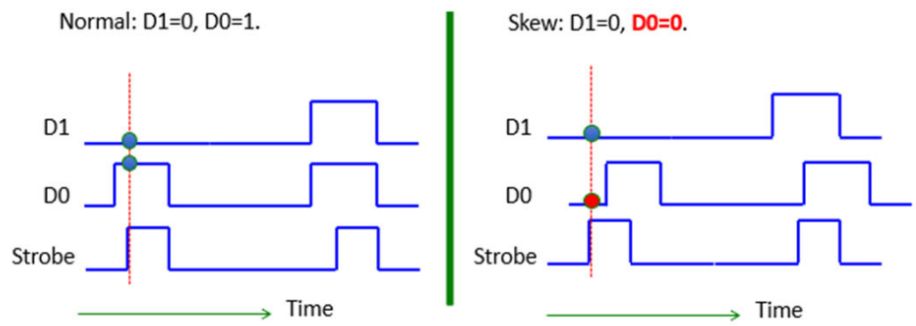
\includegraphics[width=0.4\textwidth]{images/signal-skew.png}
    \end{center}
    \item Crosstalk: Undesired coupling of signals from one circuit to another
    \begin{itemize}
        \item  Beacuse of close placement of data lines.
        \item  Interferance could be via electromagnetic domain (act like antenna) or electrical domain.
    \end{itemize}
    \item Both signal skew and crosstalk limit: the max no. of lines on the bus, max clock rate, max no. of bytes trfed in 1 block, min delay bw each byte trf.
\end{itemize}
So parallel data trf has faster data trf rate, but susceptible to signal skew and crosstalk, and higher hardware cost and bulkier.\\
\subsection*{Serial data trf}
\phantomsection
\addcontentsline{toc}{subsection}{Serial data transfer}
Data trf one bit a time, so trf rate lower compared to parallel trf, and hardware interface design more complex as it needs to handle serial to parallel conversion (processor process in bytes).\\
But able to trf data reliably over longer distance with lower cost, and less affected by signal skew and crosstalk.\\
\textbf{Serial data trf modes}
\begin{itemize}
    \item Simplex: data trf in one direction
    \item Half-duplex: data trf in both directn, but RX/TX mutually exclusive
    \item Full duplex: 2 data lines, simultaneous RX/TX
\end{itemize}
\begin{center}
    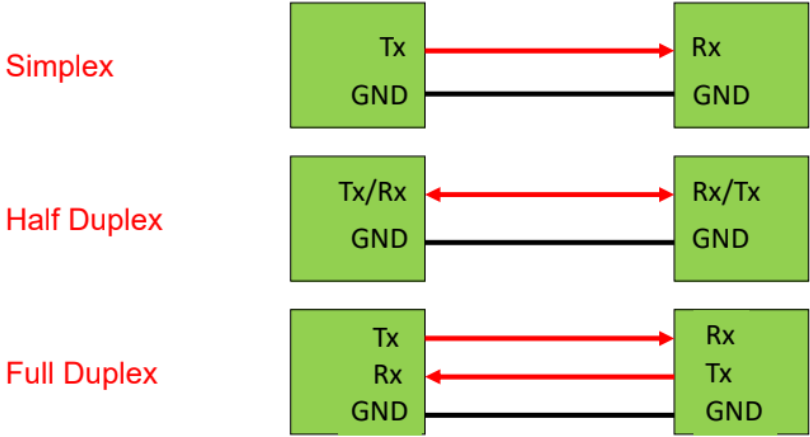
\includegraphics[width=0.35\textwidth]{images/simplex-duplex.png}
\end{center}
\textbf{Nature of communication}
\begin{itemize}
    \item Synchronous: common clock signal bw TX and RX
    \phantomsection
    \addcontentsline{toc}{subsubsection}{Synchronous transfer (SPI)}
    \begin{itemize}
        \item I2C: not tested
        \item SATA: not tested
        \item Serial Peripheral Interface (SPI) Bus.
        \begin{itemize}
            \item Initiate trf: master pulls the Slave Select (SS) low to enable the target SPI slave.
            \item Data on the Master-Out-Slave-In (MOSI) and MISO are latched on the rising edge of the SCLK signal.
            \item Multiple slaves can be connected to one master.
        \end{itemize}
        \begin{center}
            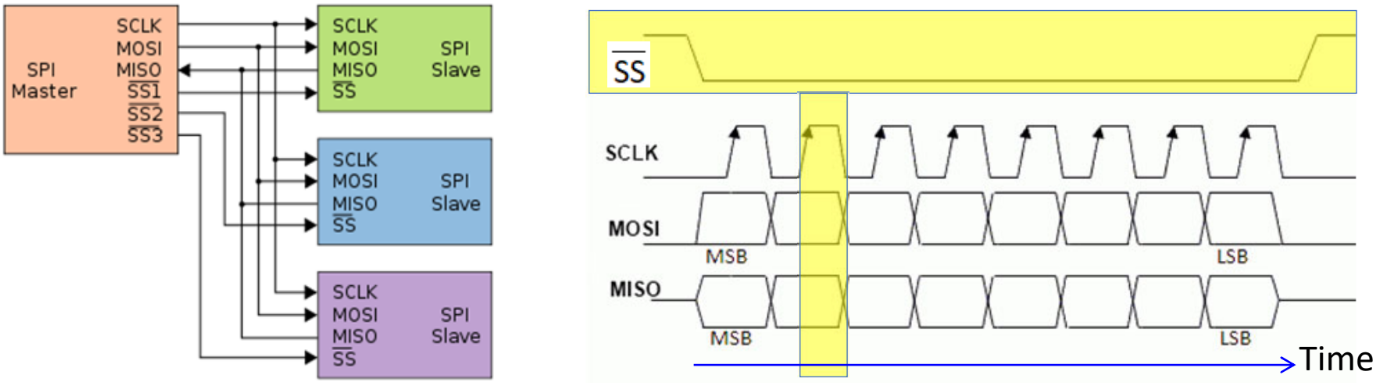
\includegraphics[width=0.4\textwidth]{images/spi-bus.png}
        \end{center}
    \end{itemize}
    \item Asynchronous: no common clock, have to agree on pre-fixede clock freq
    \phantomsection
    \addcontentsline{toc}{subsubsection}{Asynchronous data transfer (UART)}
    \begin{itemize}
        \item Universal Asynchronous Receiver Transmitter (UART)
        \begin{itemize}
            \item IDLE = logic 1.
            \item TX sends START bit (logic 0). Receiver detects the start of transmission.
            \item Then DATA is sent at some Baud rate  = no. of bits/second.
            \item PARITY bit may be sent for error checking.
            \item STOP bit (logic 1) terminates the transmission.
            \item The transmission configuration will follow DATA:PARITY:STOP. E.g. 7O1 means 7 data bits, Odd parity, 1 Stop bit.\\
            Parity can be Odd, Even, or No parity. Stop bit can be 1 or 2.
            \item LSB is sent first.
            \item Time for each bit $T = \frac{1}{\text{Baud Rate}}$.
        \end{itemize}
        \begin{center}
            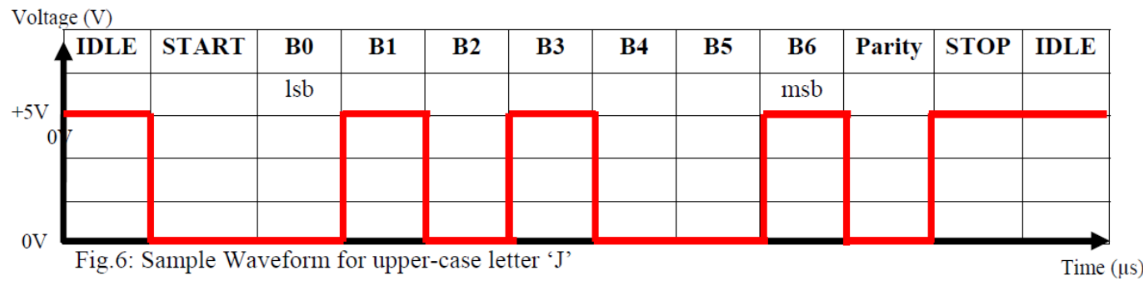
\includegraphics[width=0.4\textwidth]{images/uart.png}
        \end{center}
        \item Internal clock of UART RX will typically run a multiple times (4X here) of the baud rate, to time the sampling close to the middle of each data bit.
        \begin{center}
            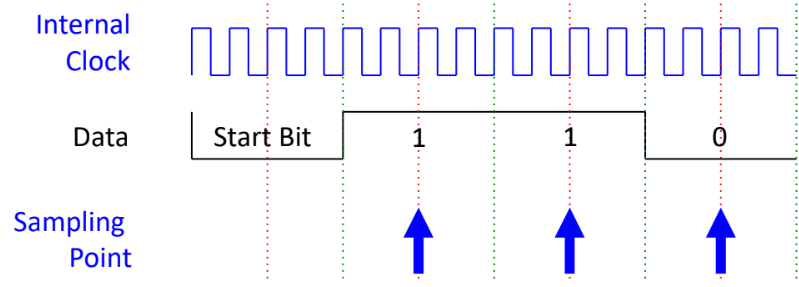
\includegraphics[width=0.3\textwidth]{images/uart-rx.png}
        \end{center}
        \item If RX samples at different baud rate, the result will be different.
        \begin{center}
            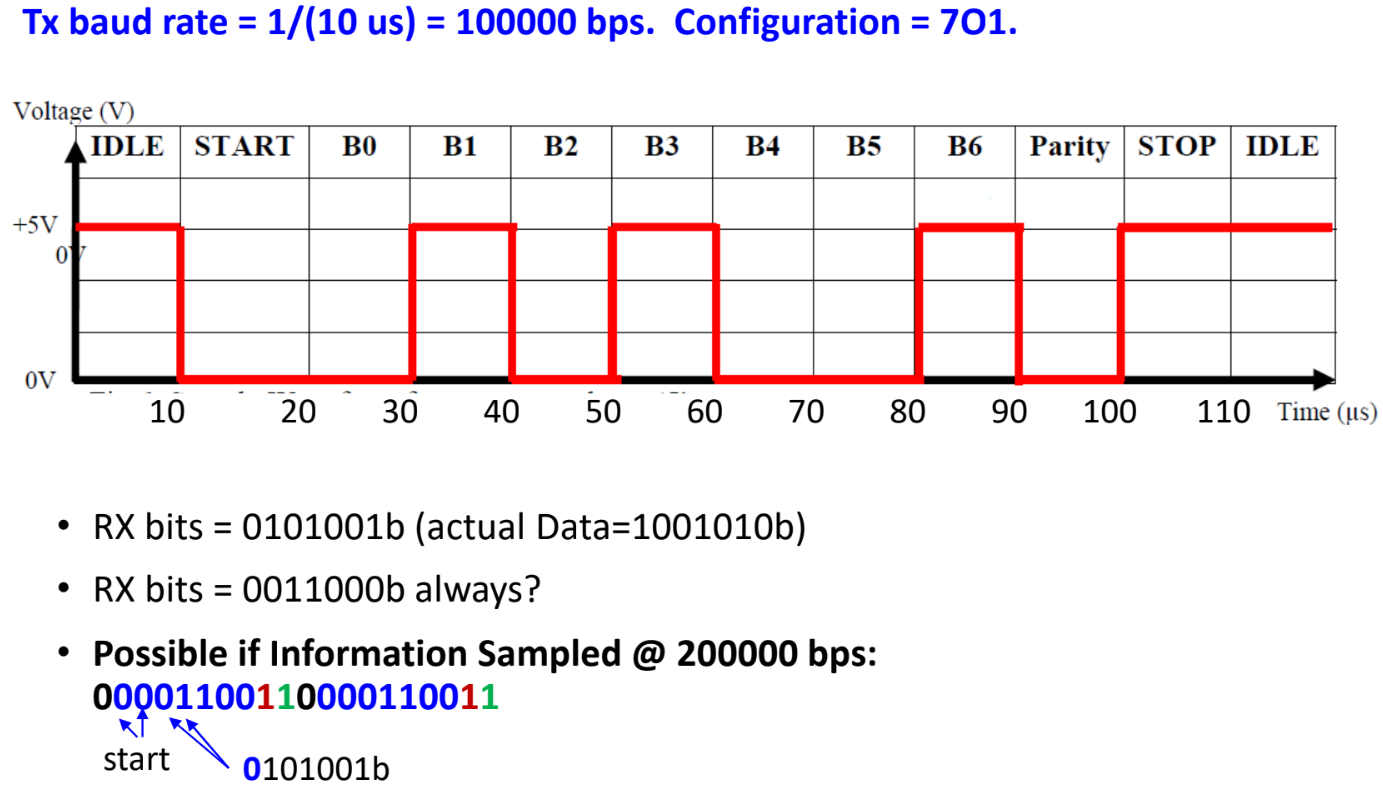
\includegraphics[width=0.4\textwidth]{images/different-baud.png}
        \end{center}
    \end{itemize}
\end{itemize}
\subsection*{Wired}
\phantomsection
\addcontentsline{toc}{subsection}{Wired}
\textbf{USB}
\phantomsection
\addcontentsline{toc}{subsubsection}{USB}
\begin{itemize}
    \item Tiered-star topology: USB host (usually the computer) connected to peripherals (e.g. mouse) directly or through USB hub.
    \begin{center}
        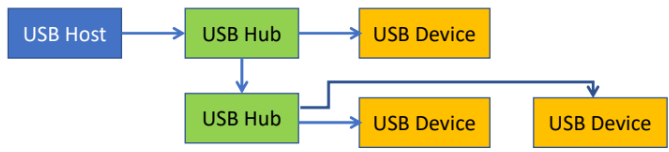
\includegraphics[width=0.4\textwidth]{images/usb-topology.png}
    \end{center}
    \item Upon connection, the host and device have to undergo enumeration (exchange info on capability \& requirement), then the host checks for device driver to support the USB device.
\end{itemize}
\textbf{High-definition Multimedia Interface (HDMI)}
\phantomsection
\addcontentsline{toc}{subsubsection}{HDMI}
\begin{itemize}
    \item Audio/video interface for transmitting uncompressed video/audio data.
\end{itemize}
\phantomsection
\addcontentsline{toc}{subsection}{Wireless}
\subsection*{Wireless}
Industrial, Scientific, Medical (ISM) radio freq (RF) bands are free-to-use frequency bands. The 2.4Ghz and 5.8Ghz bands are standard world wide.\\
\textbf{WiFi}
\phantomsection
\addcontentsline{toc}{subsubsection}{WiFi}
\begin{itemize}
    \item Operates in 2.4Ghz and 5.8Ghz RF range.
    \item Infrastructure mode: uses Star topology, at the center of the network is an Access Point or Router, connected to devices at the end.
    \item Adhoc mode: Peer to Peer connection.
    \item Transmission range generally 20m-150m.
\end{itemize}
\textbf{Bluetooth}
\phantomsection
\addcontentsline{toc}{subsubsection}{Bluetooth}
\begin{itemize}
    \item Mainly for low data rate wireless transmission, focus on low power consumption.
    \item Operates in 2.4Ghz range.
    \item Star topology.
    \item Tranmission range up to 100m but kept to 10-20m for lower power consump.
    \item 2 protocols: BT classic and BLE (Low energy), but most BT hosts can connect to both.
\end{itemize}
\textbf{Factors affecting transmission range}
\phantomsection
\addcontentsline{toc}{subsubsection}{Factors affecting transmission range}
\begin{itemize}
    \item Transmissn power: higher means greater range.
    \item Transmissn freq: higher freq, higher attenuation, lower range
    \item Interferance between closer transmitters in the same freq band.
    \begin{itemize}
        \item To mitigate, the freq band is divided into channels, and each device uses different channels.
        \item Another solution is frequency hopping from one channel to another, which is what BT uses.
    \end{itemize}
\end{itemize}

\section*{Peripherals (??)}
\phantomsection
\addcontentsline{toc}{section}{Peripherals}
\begin{itemize}
    \item Keyboard \& mouse
    \begin{itemize}
        \item Keyboard can be wired (USB) or wireless (2.4Ghz ISM), detects key presses and transmits characters by ASCII codes.
        \item Mouse primarily transmits x,y coords and left/right click.
    \end{itemize}
    \item Capacitive Touch Interface
    \begin{itemize}
        \item Touch screen works cause of change in capciitance of the hardware in presence of finger.
        This change in cap is affected by dielectric of the capacitor.
    \end{itemize}
    \item Camera
    \begin{itemize}
        \item Consists of Lens, Image sensors (convert photons to electric signals, then ADC converion for processing), Image signal processor (ISP; auto focus, exposure etc.), Interface I/O (reformatting for delivery to host processor). 
    \end{itemize}
    \item Microphones
    \begin{itemize}
        \item Use variation in capacitance when diaphragm is displaced by sound pressure to transduce sound wave to electric signals.
        \item Transduced signal is analog, but ADC can convert it to digital.
        \item ECM microphone: the charges are stored permanently on the electret.
        \item MEMs microphone: electrical charges provided by charge pump.
    \end{itemize}
    \item Liquid Crystal Display (LCD)
    \begin{itemize}
        \item Liquid crystal molecules twist the light and controls the amount of light passing through the colour filters.
        \item The orientation of these molecules controlled by electric field.
    \end{itemize}
    \item Speaker
    \begin{itemize}
        \item Electromagnetic coil moves a speaker cone, mechanical energy converted to sound.
    \end{itemize}
\end{itemize}

\phantomsection
\addcontentsline{toc}{section}{Data transfer Mechanisms}
\section*{Data Transfer Mechanisms}
Data transfer can be initiated by the CPU or the DMAC.
\phantomsection
\addcontentsline{toc}{subsection}{Polling (Programmed I/O)}
\subsection*{Polling (Programmed I/O)}
CPU polls a certain I/O port continuously (using software) for data or readiness of the port to perform a data transaction.\\
CPU uses 100\% of its resource to do the polling. It cannot entertain any other requests.
% \begin{center}
%     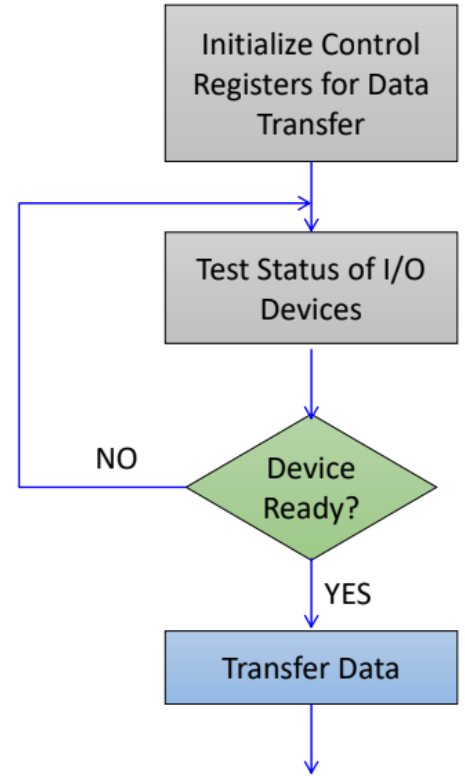
\includegraphics[width=0.15\textwidth]{images/polling.png}
% \end{center}
\clearpage
\begin{figure}[H]
    \centering
    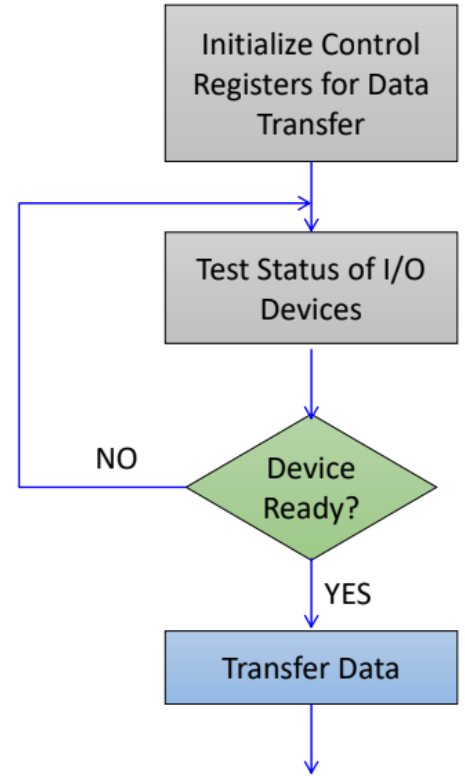
\includegraphics[width=0.15\textwidth]{images/polling.png}
\end{figure}
\begin{itemize}
    \item Programmer has complete control over the process, easier to test and debug.
    \item Program execution of CPU held up while waiting for I/O device to get ready, inefficient use of CPU resources.
\end{itemize}
\subsection*{Interrupt Triggered}
\phantomsection
\addcontentsline{toc}{subsection}{Interrupt Triggered}
\begin{itemize}
    \item Uses hardware: A signal from external/internal peripheral, or a change in status of some special registers notifies the CPU that some event has occur.
    \item If the CPU decide to service the interrupt, it will suspend its current program temporarily.
    \item The interrupt will come with some interrupt vector table (IVT) index.
    \item CPU look up the IVT to check the starting address of the interrupt service routine (ISR) for the corresponding interrupt.
    \item CPU then proceed to execute the ISR linked to the interrupt that was triggered (typically a short routine).
    \item Once the ISR is completed, CPU restore the saved context, returns to the interrupted routine and continue from where it had left previously.
    \item \textbf{Interrupt latency}: delay bw CPU receiving the interrupt req, and the pt of entering the ISR.
\end{itemize}
\begin{center}
    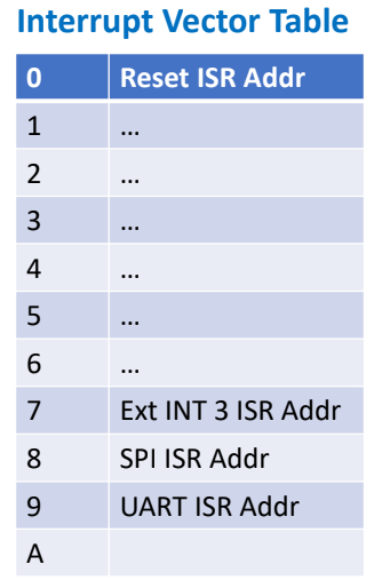
\includegraphics[width=0.1\textwidth]{images/ivt.png}
\end{center}
\begin{itemize}
    \item CPU does not need to monitor I/O device status, more efficient use of CPU resources.
    \item But more hardware interface circuitry required between I/O device and processor. Program is slightly more complex and difficult to debug.
\end{itemize}
\subsection*{Direct Memory Access (DMA)}
\phantomsection
\addcontentsline{toc}{subsection}{Direct Memory Access (DMA)}
DMAC is a Data Bus Controller module that performs data transfer independent of CPU.
\begin{center}
    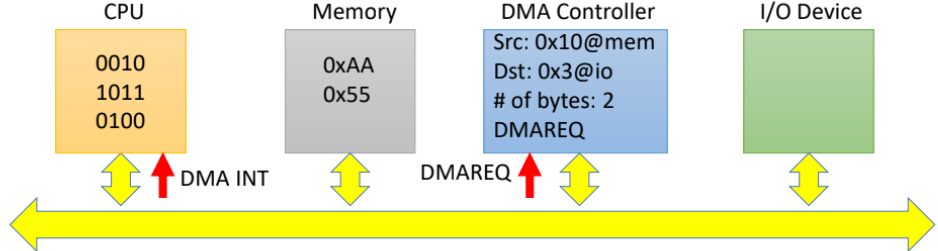
\includegraphics[width=0.4\textwidth]{images/dmac.png}
\end{center}
\begin{itemize}
    \item CPU configures some parameters for DMAC to trf data
    \begin{itemize}
        \item Src and Dest addr of data
        \item No. of bytes to trf
        \item Trigger signal telling DMAC when to start the trf.
    \end{itemize}
    \item DMAC waits till trigger signal comes in.
    \item It requests for system bus and start data trf. (Data goes into internal buffer of DMAC before transferred to dest)
    \item After trf, DMAC releases the system bus, notifies CPU of data completion via interrupt. 
\end{itemize}
3 modes of transfer:
\begin{itemize}
    \item Burst: During control of the system bus, DMAC trf multiple units of data.
    \phantomsection
    \addcontentsline{toc}{subsubsection}{Burst}
    \begin{itemize}
        \item Could be entire block of data that DMAC tasked to trf, or just a subset of that block.
        \item CPU can continue with its operation as long it does not need the particular system bus that DMAC is using.
        \item So Burst has faster trf rate but CPU may be suspended/inactive if CPU has to wait for DMAC to complete its trf.
    \end{itemize}
    \item Cycle stealing: DMAC trfs one unit of data aft taking control, then releases control of system bus to CPU.
    \phantomsection
    \addcontentsline{toc}{subsubsection}{Cycle stealing}
    \begin{itemize}
        \item DMAC can execute the data trf between CPU instructions or between pipeline stages.
        \item CPU may be suspended if it need to access the system bus but suspend time is shorter as only one unit is transferred at one time.
        \item Transfer rate is slower than in Burst Mode but will CPU will only be inactive for very short period of time.
        \item Favoured if CPU needs to be responsive.
        \begin{center}
            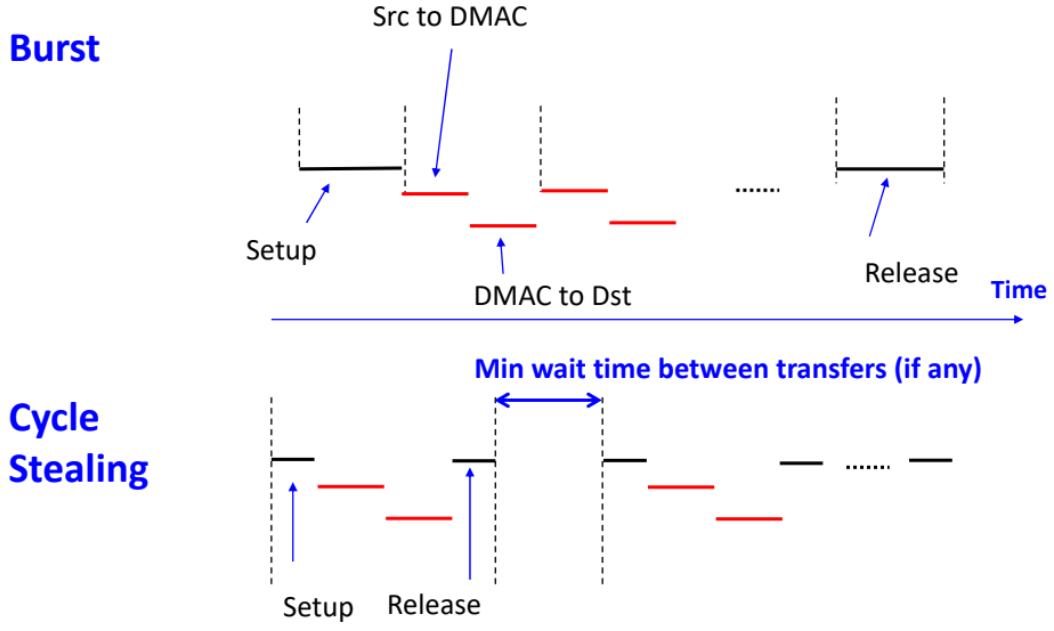
\includegraphics[width=0.4\textwidth]{images/burst-cycle-stealing.png}
        \end{center}
    \end{itemize}
    \item Transparent: DMAC trfs data only when CPU not using the system bus.
    \phantomsection
    \addcontentsline{toc}{subsubsection}{Transparent}
    \begin{itemize}
        \item CPU performance not affected, but potentially slowest trf rate.
        \item More complex hardware needed to detect when CPU not using the system bus.
    \end{itemize}
    \item So from burst to cycle-stealing to transparent, data trf gets slower but CPU performance/response improves.
    \item Transferring via CPU can be faster than DMA as CPU speed is typically faster, just that it means wasting CPU resources to just transfer data.
\end{itemize}

\section*{Memory}
\phantomsection
\addcontentsline{toc}{section}{Memory}
\subsection*{Volatile}
\phantomsection
\addcontentsline{toc}{subsection}{Volatile}
Data lost when electric power is removed. Used as system memory.
\begin{itemize}
    \item \textbf{Static Random Access Memory (SRAM)}
    \phantomsection
    \addcontentsline{toc}{subsubsection}{SRAM}
    \begin{itemize}
        \item Large, 4-6 transistors per cell.
        \item Fast, optimised for speed/access latency.
        \item Low power consumption.
    % \begin{center}
    %     \fbox{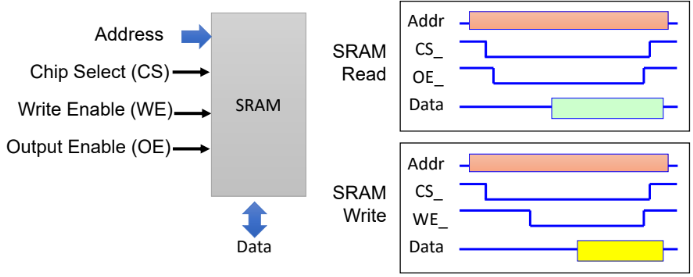
\includegraphics[width=0.4\textwidth]{images/sram-access.png}}
    % \end{center}
    \vspace{1ex}
    \noindent\makebox[\linewidth]{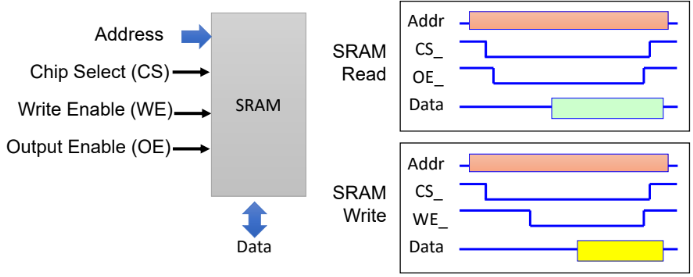
\includegraphics[width=0.9\linewidth]{images/sram-access.png}}
    \vspace{1ex}    
        \item One chip can contain 1M SRAM cells. Each SRAM contains 6 transistors.
        \begin{itemize}
            \item Word Line (WL) controls which cells are enabled for read \& write.
            \item Bit Lines (BL) carry the actual data.
            \item M1, M2, M3, M4 stores the data bit (equivalent to the 2 invertors: the logic state that is stored remains unchanged so long as the gates are powered).
            \item M5, M6 are pass (switch) transistors, controls the cell to be connected for read/write operation.
        \end{itemize}
        \clearpage
        \begin{center}
        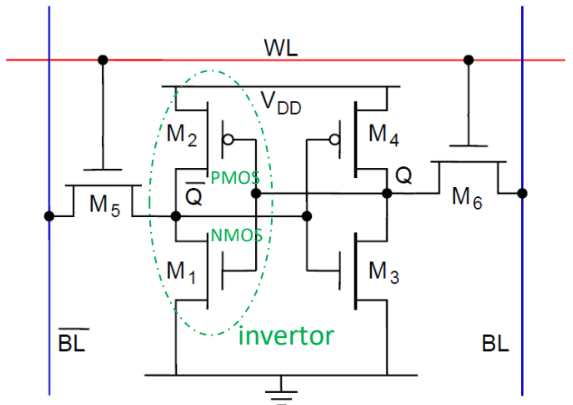
\includegraphics[width=0.3\textwidth]{images/sram-transistors.png}
        \end{center}
    \begin{center}
        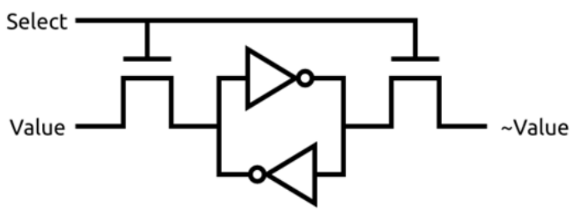
\includegraphics[width=0.25\textwidth]{images/sram-logic.png}
    \end{center}
        \item Best for implementing cache as cache needs fast memory.
    \end{itemize}
    \item \textbf{Dynamic RAM (DRAM)}
    \phantomsection
    \addcontentsline{toc}{subsubsection}{DRAM}
    \begin{itemize}
        \item Small, 1-3 transistors per cell. (Less transistors doesn't imply simpler interface design!)
        \item Slower, optimised for density/higher capacity.
        \item Requires periodic refresh (because of capacitor), higher power consumption.
        \begin{center}
            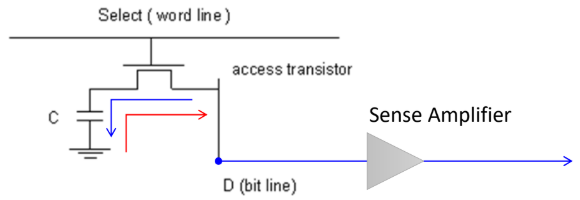
\includegraphics[width=0.4\textwidth]{images/dram.png}
        \end{center}
        \item DRAM cell contains 1 transistor \& 1 capacitor.
        \begin{itemize}
            \item Store logic '1' (blue): enable transistor, transfer charge into capacitor.
            \item Store logic '0' (red): enable transistor, discharge capacitor.
            \item Read: enable transistor, measure capacitor charge using sense amplifier.
        \end{itemize}
        \item Reading process destroys data, so the original data has to be written back after every read.
        \item Periodic refresh is needed as the charges leak over time.
        \item Modern version of DRAM is SynchronousDRAM (SDRAM)
        \begin{itemize}
            \item uses clock signal from host to synchronise data transfer.
            \item employs pipeline architecture that allows faster, overlapping operations.
        \end{itemize}
    \end{itemize}
\end{itemize}
\subsection*{Non-volatile}
\phantomsection
\addcontentsline{toc}{subsection}{Non-volatile}
Data is retained even if electric power is removed. Used as storage memory.\\
\textbf{Floating Gate Transistor (FGT)}\\
\phantomsection
\addcontentsline{toc}{subsubsection}{FGT}
\begin{center}
    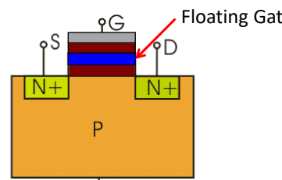
\includegraphics[width=0.2\textwidth]{images/fgt.png}
\end{center}
\begin{center}
    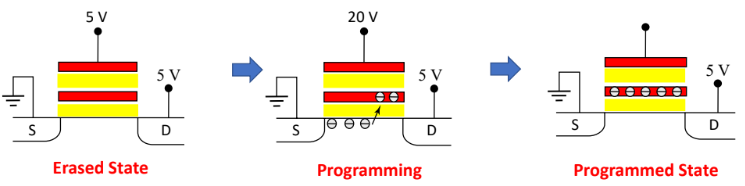
\includegraphics[width=0.5\textwidth]{images/fgt-states.png}
\end{center}
\begin{itemize}
    \item To program the FGT, a large +ve voltage is applied to the gate.
    \item Some electrons tunnel through the oxide and embed into the floating gate.
    \item In the programmed state, the excess electrons in the floating gate will continue to be trapped there even if the power is removed.
\end{itemize}
\begin{center}
    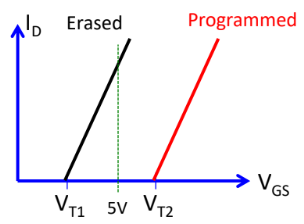
\includegraphics[width=0.2\textwidth]{images/fgt-threshold.png}
\end{center}
\begin{itemize}
    \item FGT becomes conductive when gate voltage (V$_{\text{GS}}$) above the threshold voltage (V$_{\text{T}}$).
    \item In the programmed state, the excess -trons in the floatg gate lower the voltage potential, so a larger voltage is needed to attract enough electrons to form the conductive layer.
    \item Hence we can perform these operations on FGT:
    \begin{itemize}
        \item Read content: apply voltage between the two thresholds. If FGT ON, it is in erased state (bit '1'). If OFF, it is programmed state (bit '0').
        \item To write '1': erase the FGT (using UV light or electrically).
        \item To write '0': program the FGT.
    \end{itemize}
    \item In practice, after a flash is erased, it contains all '1's in memory. Programming stores '0's.
    \item To write data to a memory location and bits need to be changed, the whole block (multiple bytes) is erased to '1's, then programming sets some of the '1's to '0's.
\end{itemize}
\textbf{Erasable Programmable Read-Only Memory (EPROM) / Electrically Erasable PROM (EEPROM)}\\
\phantomsection
\addcontentsline{toc}{subsubsection}{EPROM/EEPROM}
Implementation of the FGT.\\
\begin{itemize}
    \item EPROM requires UV light to erase the stored program. Legacy technology.
    \item EEPROM can be electrically erased.
    \item Compared to Flash, smaller page size (tens of bytes) and larger erase cycle endurance (can tolerate larger no. of erasures before failing).
    \item Higher cost per bit.
\end{itemize}
\textbf{Flash}\\
\phantomsection
\addcontentsline{toc}{subsubsection}{Flash}
Uses FGT technology.\\
\begin{itemize}
    \item Can be erased in larger blocks compared to EEPROM.
    \item Faster speed than EEPROM when performing write operations.
    \item Costs less per bit.
\end{itemize}

\textbf{NOR Flash}\\
\phantomsection
\addcontentsline{toc}{subsubsection}{NOR Flash}
Used mainly as system memory.\\
Has multiple Address and Data lines.
\begin{center}
    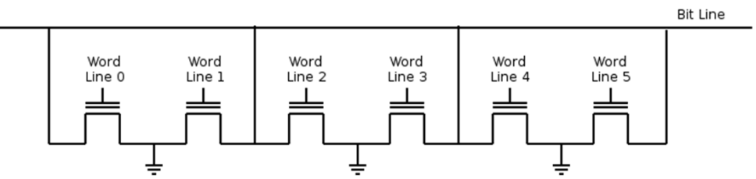
\includegraphics[width=0.4\textwidth]{images/nor-flash.png}
\end{center}
FGT cells are connected to resemble NOR gate logic.\\
To read, the CPU sends voltage down the specific Word Line, and the transistor either turns ON or stays OFF, depending on erased or programmed state.
\begin{itemize}
    \item If erased state, current flows from Bit Line into Ground, so the sense amplifier detects this as logic 1.
    \item If programmed state, no current flows from Bit Line, detected as Logic 0.
\end{itemize}
NOR flash supports XIP (execute-in-place): Code can be executed directly from flash memory without loading the code into RAM (main memory).
\begin{itemize}
    \item This is possible as NOR flash allows random reading, i.e. can read data using only address information.
\end{itemize}
So we have the following operations for NOR flash:
\begin{itemize}
    \item Reading: Very fast.
    \item Writing (programming): require the high voltages to program the FGTs, one byte at a time.
    \item Erasing: Done at block level.
\end{itemize}
\textbf{NAND Flash}\\
\phantomsection
\addcontentsline{toc}{subsubsection}{NAND Flash}
Has only one I/O bus so all Commands, Addresses, Data has to go through this bus.\\
Data is accessed a page at a time. Command used to open a particular page followed by the individual bytes read/write.
\begin{center}
    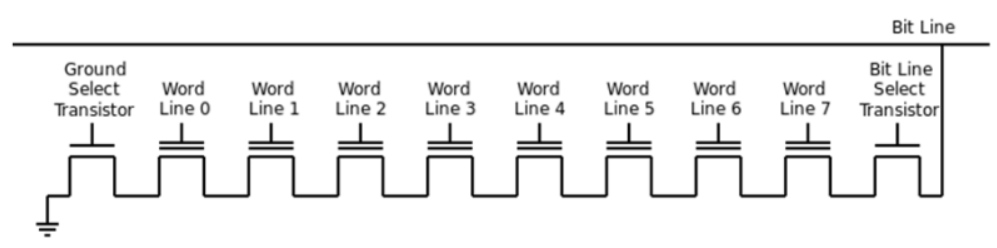
\includegraphics[width=0.4\textwidth]{images/nand-flash.png}
\end{center}
FGT cells are connected to resemble NAND gate logic.\\
To read Word Line 3, 
\begin{itemize}
    \item the system first applies a huge voltage to the transistors we don't want to read.
    \item This voltage is so high that it forces them to turn ON, regardless of what data they are holding.
    \item Then, it applies the normal "Read Voltage" to the specific transistor you do want to read (Word Line 3) to see if it turns on or stays off.
\end{itemize}
NAND does not support XIP. E.g. for read op,
\begin{itemize}
    \item CPU first sends a Command telling the NAND flash what operation to be carried out.
    \item CPU then sends the address.
    \item The NAND chip reads an entire page. (page contains multiple bytes, block contains multiples pages).
\end{itemize}
Why use NAND flash? Less connecting wires, higher density, lower cost per bit, used for main storage like SSD, USB.\\
\textbf{Hard Disk Drive (HDD)}
\phantomsection
\addcontentsline{toc}{subsubsection}{HDD}
\begin{center}
    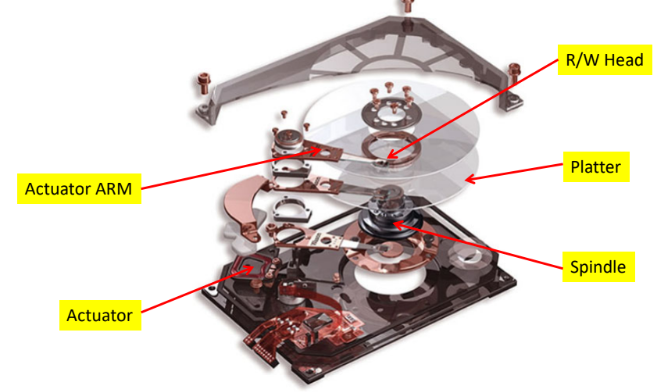
\includegraphics[width=0.4\textwidth]{images/hdd.png}
\end{center}
\begin{center}
    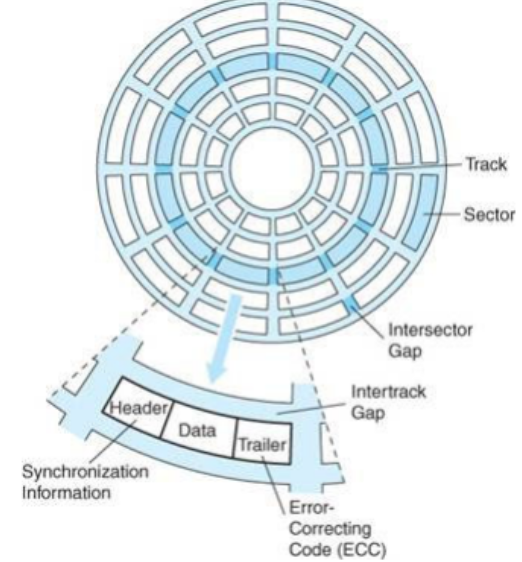
\includegraphics[width=0.2\textwidth]{images/hdd-sectors.png}
\end{center}
Platters rotate on the spindle. Each platter has two surfaces. Each surface is served by a R/W head.\\
    Data is stored on the platters, which is organised in concentric rings called \textbf{tracks} or \textbf{cylinders}.\\
Tracks are divided into \textbf{sectors}, each containing header, data and trailer.
\begin{center}
    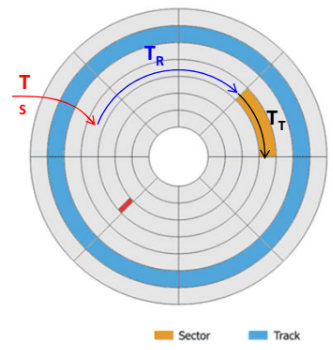
\includegraphics[width=0.2\textwidth]{images/hdd-times.png}
\end{center}
Note that the platter is always spinning.
\begin{itemize}
    \item Define RPS = RPM / 60.
    \item Seek Time $T_S$: Time taken for RW head to swing such that it hovers over the specific Track.
    \item Rotational Delay $T_R$: Time taken for platter to spin until the target sector pass under the RW head.\\
    On average, $$T_R = \frac{0.5}{RPS}s$$
    \item Access Time $T_A$: $T_S$ + $T_R$
    \item Transfer Time $T_T$: Time taken for the sector to sweep past the head, during which the RW head interacts with the magnetic fields of the magnetic domains to read/write.\\
    Defining the track density $D_T$ (no. of sectors/track) and sector density $D_S$ (no. of bytes/sector), and the no. of bytes $N$ for the transfer, then
    $$T_T = \frac{N}{RPS\times D_T \times D_S}$$
    \item Usually, $T_A \gg T_T$, so if data is spread across different sectors in diff tracks, the effective HDD trf rate drops a lot. Defragmentation will bytes of a file in consecutive sectors.
    \item $T_T=\frac{1}{RPS}$ for one full track.
\end{itemize}
\begin{center}
    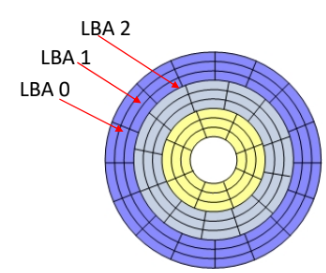
\includegraphics[width=0.2\textwidth]{images/hdd-modern-layout.png}
\end{center}
\begin{itemize}
    \item Early HDD had equal no. of sectors per track, which wastes space as bit density of those sectors are not optimal.
    \item Logical layout used Cylinder-Head-Sector (CHS), but obselete now due to limitation in HDD capacity it can support.
    \item Modern HDD implements zone bit recording, where tracks are divided into zones, with differing no. of sectors per track for diff zones.
    \item Modern logical layout uses Logical Block Addressing (LBA): the first block in HDD has addr LBA0, next LBA1, so on. 48 bits allocated to specify this number.
\end{itemize}
\textbf{Solid state drive (SSD)}
\phantomsection
\addcontentsline{toc}{subsubsection}{SSD}
\begin{center}
    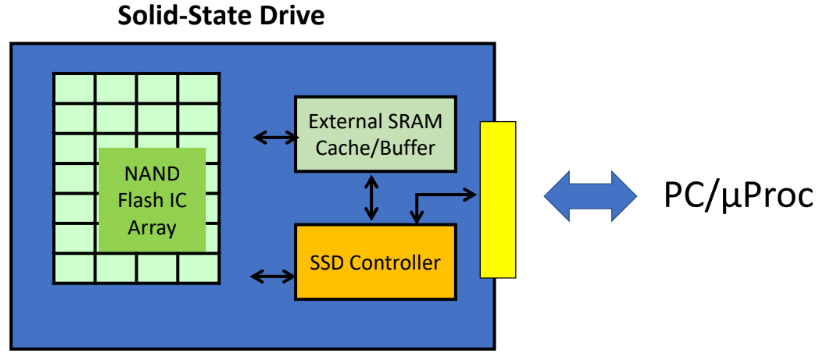
\includegraphics[width=0.4\textwidth]{images/ssd.png}
\end{center}
\begin{itemize}
    \item Main storage element in SSD is NAND flash.
    \item Flash memory has limited program-erase cycles. Techniques to extend life of SSD:
    \begin{itemize}
        \item Wear levelling: distributing data erase/write operations evenly over the entire disk.
        \item Use external RAM as buffer to minimise the no. of writes to Flash.
        \item Error correction code: ability to recover from one or more bits of error in media.
    \end{itemize}
    \item The SSD controller is a microprocessor, which handles address translation b/w logical \& physical layout, caching and buffering out of the SSD, and wear levelling algorithm.
    \item External SRAM and cache improve the trf rate for r/w ops.
\end{itemize}
\textbf{HDD vs SSD}:
\phantomsection
\addcontentsline{toc}{subsubsection}{HDD vs SSD}
\begin{itemize}
    \item HDD has lower cost per bit and almost infinite erasure cycles.
    \item But HDD has many moving parts, vulnerable.
    \item SSD more expensive, but higher trf rate and smaller form factor than HDD.
    \item But SSD has limit on no. of erasure cycles. Some techniques to mitigate:
    \begin{itemize}
        \item Wear levelling - extend life of SSD by distributing erase/write ops evenly over the entire disk.
        \item use ext RAM as buffer to minimise no. or writes to flash in SSD.
    \end{itemize}
    \item HDD is still the dominant storage in data centres, because there is huge cost difference.
\end{itemize}

\section*{Cache}
\phantomsection
\addcontentsline{toc}{section}{Cache}
\begin{center}
    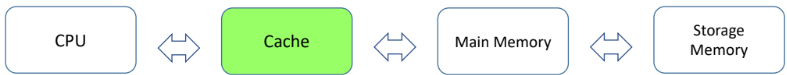
\includegraphics[width=0.4\textwidth]{images/cache.png}
\end{center}
Cache is a fast memory, act as buffer between CPU and MM.
\begin{itemize}
    \item Best implemented with SRAM. DRAM is too slow and its trf procedure is too complex for cache ops. Flash is not suitable due to finite erase cycles and slower speed.
\end{itemize}
CPU first checks cache, then main memory and finally system memory.\\
A subset of the code and data that is frequently used is stored in cache.\\
\subsection*{Principle of Locality}
When a byte of code/data is accessed in a program, it is very likely that nearby code or data will be needed soon.
\phantomsection
\addcontentsline{toc}{subsection}{Principle of Locality}
\begin{itemize}
    \item Locality of space: code/data near each tgt likely to be accessed tgt, so transfers between cache and main memory happen in blocks.
    \item Locality of time: recently used code/data likely to be used again. Used when designing cache replacement policy.
\end{itemize}
\subsection*{Direct mapped cache}
\phantomsection
\addcontentsline{toc}{subsection}{Direct mapped cache}
\begin{figure}[H]
    \centering
    % First image minipage
    \begin{minipage}[b]{0.2\textwidth}
        \centering
        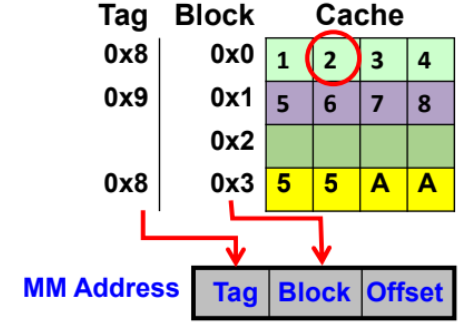
\includegraphics[width=\textwidth]{images/direct-map-cache.png}
        % \caption{Caption for Figure 1}
    \end{minipage}
    \hfill % Pushes the minipages apart
    % Second image minipage
    \begin{minipage}[b]{0.2\textwidth}
        \centering
        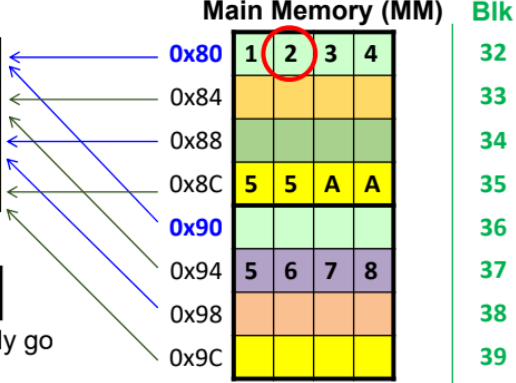
\includegraphics[width=\textwidth]{images/direct-map-cache-2.png}
        % \caption{Caption for Figure 2}
    \end{minipage}
\end{figure}
\begin{itemize}
    \item Each main memory block can only go to 1 specific block in cache.
    \item The main memory address can be partitioned into TAG:BLK:OFFSET.
    \begin{itemize}
        \item OFFSET = no. of bits needed to represent cache block size. 4 byte block size = 2 bits for OFFSET.
        \item BLK = no. of bits to represent no. of cache blocks. 4 cache blocks = 2 bits for BLK.
        \item TAG = the remaning no. of bits. The unique identifier for each MM block. 
    \end{itemize}
    \item Note that MM physical address is used as the basis. 
    \item Data retrieval from cache:
    \begin{enumerate}
        \item Derive the block number from address.
        \item Check the TAG associated with that block. If it matches the address we want to retrieve from, it is Cache Hit. Otherwise, it's a Cache Miss.
        \begin{itemize}
            \item If Cache Hit, CPU will retrieve the data and proceed.
            \item If Cache Miss, the corresponding MM block will be trf into the block.
        \end{itemize}
    \end{enumerate}
    \item DMC does not need cache replacement policy as the mapping is one-to-one.
    Some policies are Least Recently Used algorithm and FIFO approach.
    \item When the CPU writes to the cache (causing Dirty Blocks), it can either be Write Hit or Write Miss.
    \begin{itemize}
        \item Write Hit: Can implement Write Through (update cache and MM simultaneously) or Write Back (update MM only when cache block selected for replacement).\\
        Trade off between overloading system bus and cache coherency issue.
        \item Write Miss: Can implement Write Allocate (corresponding MM block will be loaded into Cache, allowing future R/W) or Write-no-allocate (CPU just writes directly to MM block, and cache is not updated).
    \end{itemize}
    \item Effective Access Time: With $H$ as the Cache Hit Rate, and assuming a sequential access of cache and MM,
    $EAT = H \times \text{Access}_C + (1-H) \times (\text{Access}_C + \text{Access}_{MM})$
\end{itemize}

\section*{Virtual Memory}
\phantomsection
\addcontentsline{toc}{section}{Virtual Memory}
Each program has its own Virtual Memory Space.\\
The OS converts virtual memory to physical memory.\\
Virtual Memory allows for
\begin{itemize}
    \item More capacity - can run more applications at once than physical RAM can hold.
    \item Every program has its own virtual memory space, so programs cannot overwrite each other's memory.
    \item Virtual addresses can seem contiguous when it is actually fragmented in physical memory.
\end{itemize}
\subsection*{Paging with Page Table}
\phantomsection
\addcontentsline{toc}{subsection}{Paging with Page Table}
\begin{itemize}
    \item Virtual Memory space is partitioned into Pages.
    \item Physical memory partitioned into Frames.
    \item Pages are mapped to frames in a page table.
    \begin{center}
        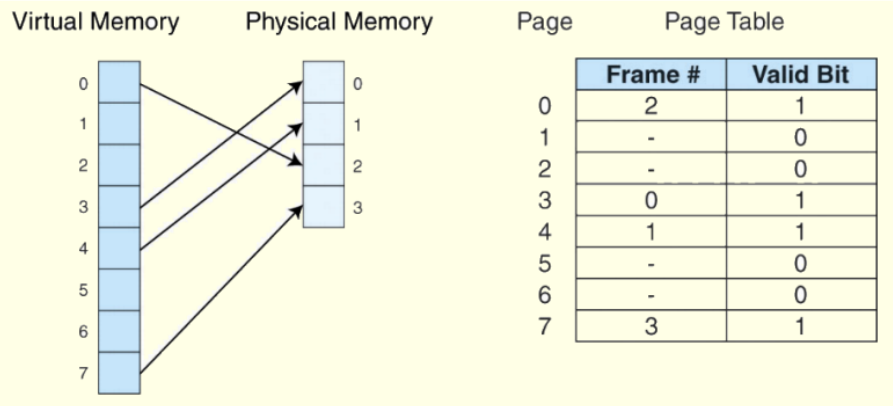
\includegraphics[width=0.4\textwidth]{images/page-table.png}
    \end{center}
    \item In the page table, every page (virtual) has a row. If mapped to a frame, the frame no. will show, and the valid bit will be '1' if it is valid mapping.
    \begin{center}
        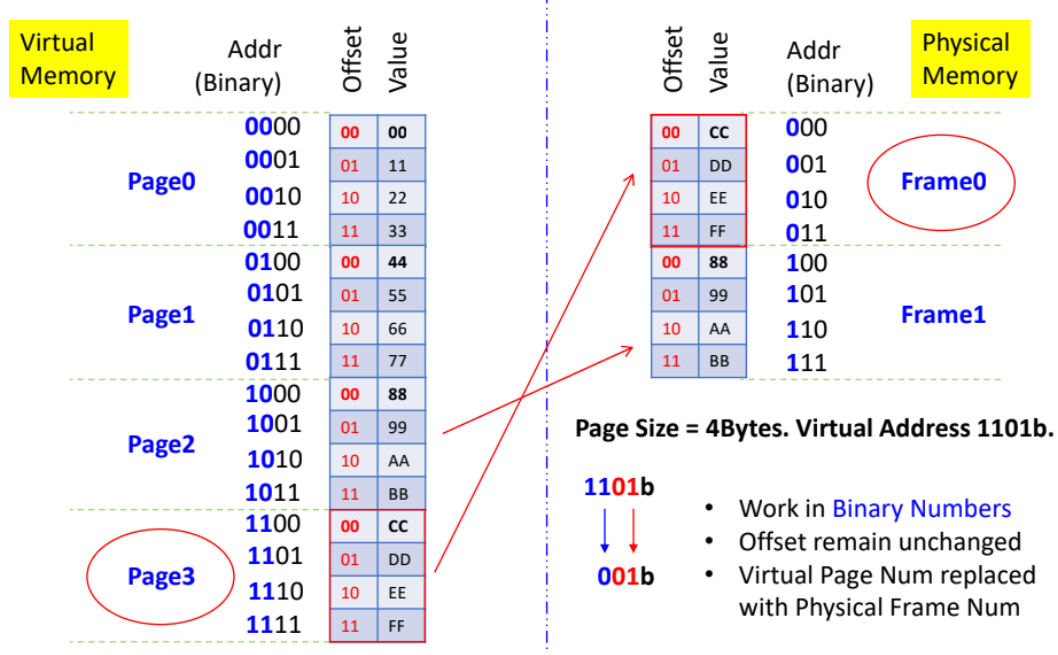
\includegraphics[width=0.3\textwidth]{images/addr-translation.png}
    \end{center}
    \begin{center}
        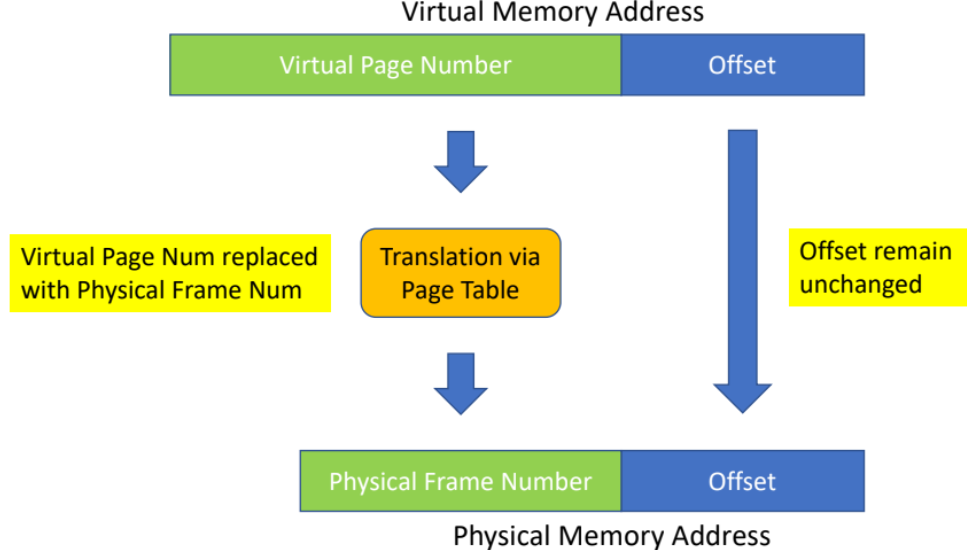
\includegraphics[width=0.3\textwidth]{images/virtual-to-physical.png}
    \end{center}
    \item Virtual address partitioned into PAGE:OFFSET, physical mem partitioned into FRAME:OFFSET.
    \item The offsets within a page are unchanged when mapped to a frame. OFFSET can be calculated by page size or frame size.
    \item Then just replace the PAGE bits with FRAME bits from page table.
    \item Page Fault occurs when a page has no mapping to a frame in MM (valid bit = 0). The OS is triggered to load the data from storage mem to MM.
    \begin{center}
        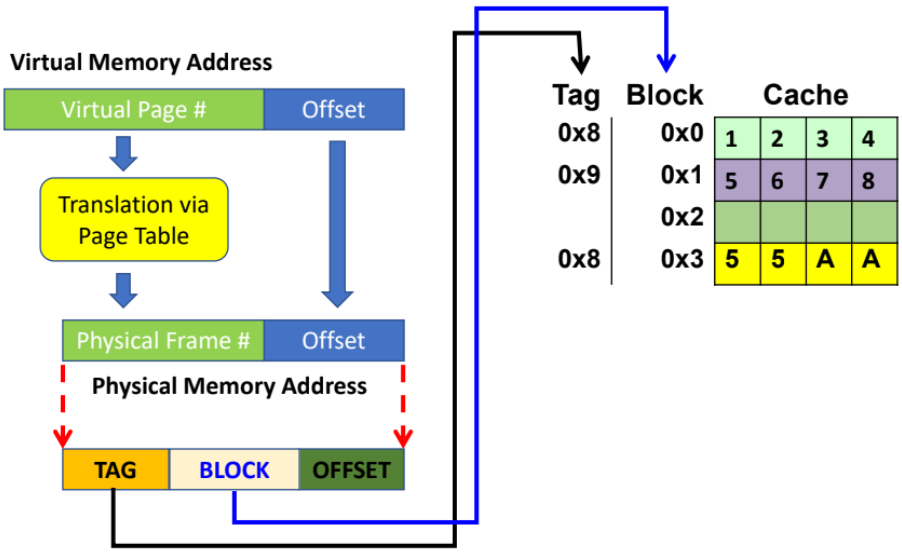
\includegraphics[width=0.3\textwidth]{images/vm-cache.png}
    \end{center}
    \item If Cache uses physical memory, then virtual address need to be converted before checking cache.
    \item If Cache uses virtual memory, then CPU checks cache first. If cache hit, CPU retrieves data and proceeds. Else, OS has to translate to physical memory first addr before fetching the required data from main memory.
\end{itemize}
\subsection*{TLB}
\phantomsection
\addcontentsline{toc}{subsection}{TLB}
\begin{itemize}
    \item Translation Lookaside Buffer (TLB) is in the CPU, stores subset of the Page Table info. Functions like a cache to the Page table, if TLB hit rate is high, overall speed of address translation will increase.
    \item All entries in the TLB are valid.
    \begin{center}
        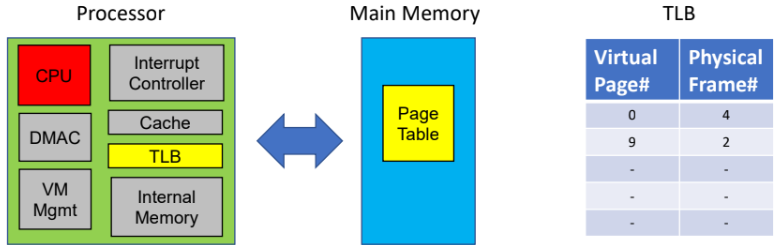
\includegraphics[width=0.4\textwidth]{images/tlb.png}
    \end{center}
\end{itemize}

\section*{Pipeline}
\phantomsection
\addcontentsline{toc}{section}{Pipeline}
\textbf{Pipelining}: partition an instruction into simpler stages (like Fetch-Decode-Execute) and assigning indep resources so these stages can execute simultaneously.\\
E.g. Executing 3 instructions takes 5 clock cycles instead of 9.\\
\subsection*{Pipeline conflict}
\phantomsection
\addcontentsline{toc}{subsection}{Pipeline conflict}
\begin{enumerate}
    \item \textbf{Resource conflict}: two instructions attempt to access the same resource in the same clock cycle.
    \phantomsection
    \addcontentsline{toc}{subsubsection}{Resource conflict}
    \begin{itemize}
        \item E.g. F-D-E-S: Instruction1 wants to store data (using system bus) while instruct4 wants to fetch instruction (using the same system bus).
        \item \textbf{Solution}: Have sufficient resources, like multiple internal buses, processing units like ALUs etc.
    \end{itemize}
    % \vspace{-0.5cm}
    % \begin{figure}[H]
    %     \centering
    %     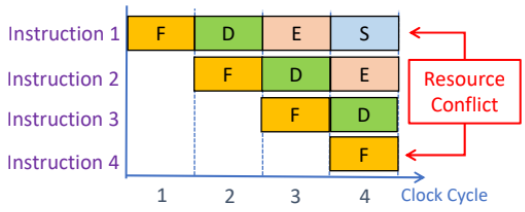
\includegraphics[width=0.3\textwidth]{images/resource-conflict.png}
    %     % \caption{This is a description of the image.}
    %     \label{fig:my_image}
    % \end{figure}
    \begin{center}
        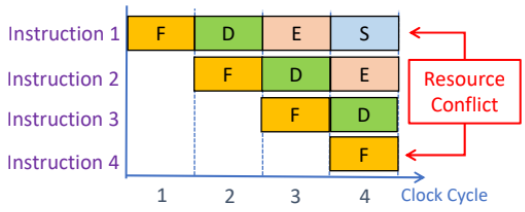
\includegraphics[width=0.3\textwidth]{images/resource-conflict.png}
    \end{center}
    % \vspace{-0.5cm}
    \item \textbf{Data dependency conflict}: Instructions overlap \& the destination operand of instruct1 may be the source operand of instruct2 $\to$ that operand may not be updated when instruct2 executes.
    \phantomsection
    \addcontentsline{toc}{subsubsection}{Data dependency conflict}
    \begin{itemize}
        \item E.g. F-D-E-S: instruct1 (\texttt{ADD R2, R2, R1}), instruct2 (\texttt{SUB R3, R3, R2}); at the start of E for instruct2, R2 is not updated (only updated at end of S of instruct1).
        \item \textbf{Solution 1}: Hardware detects data dependency (by comparing dest identifier in E stage with sources in the D stage), and stalls the E stage of subsequent instruction for one cycle (to allow the overlapped operand to be updated).
        % \vspace{-1cm}
        \begin{figure}[H]
            \centering
            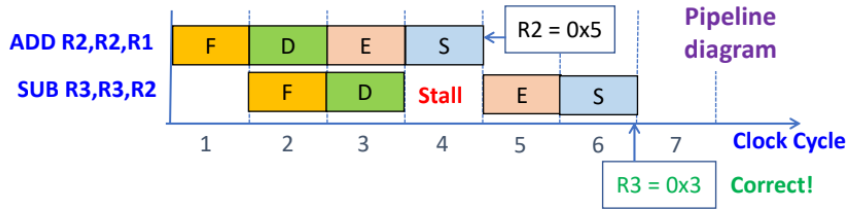
\includegraphics[width=0.4\textwidth]{images/pipeline-stall.png}
            % \caption{This is a description of the image.}
        \end{figure}
        % \vspace{-1cm}
        \item \textbf{Solution 2}: Compiler inserts \texttt{NOP} (no operation) instructs betwen instruct with data dependencies, at compilation time. Total execution time increases.
        \begin{center}
            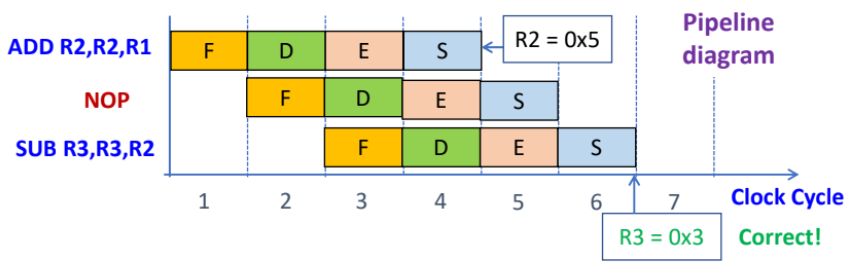
\includegraphics[width=0.4\textwidth]{images/nop-instruct.png}
        \end{center}
    \end{itemize}
    \item \textbf{Branch instruction}: The branch target is only known after E stage of branch instructions. By this time, the next 2 instructions would have been fetched (during the D and E stage of B instruct).
    \phantomsection
    \addcontentsline{toc}{subsubsection}{Branch instruction}
    \begin{itemize}
        \item If the branch is true, the two instructs are discarded, resulting in 2-cycle branch delay, and the 2 slots are Delay Slots.
        \item (Ignoring pipeline conflicts) Calculation of Total Cycles = Total Instructions + (Pipeline Depth - 1) + Wasted Cycles        
        \begin{center}
            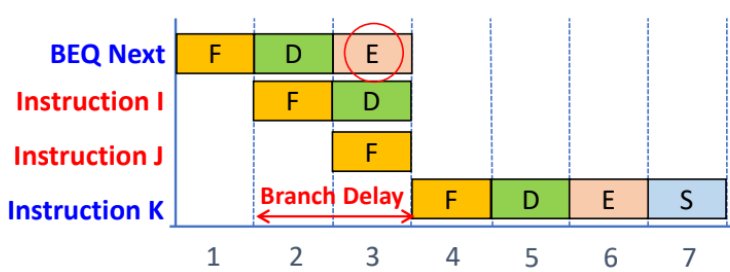
\includegraphics[width=0.35\textwidth]{images/branch-delay.png}
        \end{center}
        \item \textbf{Solution 1}: Reduce branch delay - introduce an additional adder during D stage of B instruct, to calc the branch target earlier. If branch is true, only 1 instruct discarded, so 1-cycle branch delay.
        \begin{center}
            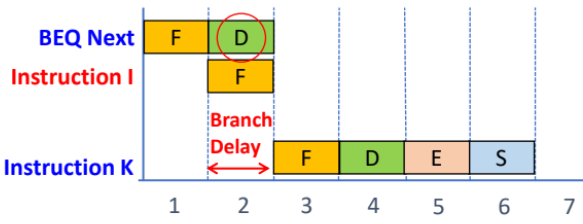
\includegraphics[width=0.3\textwidth]{images/decode-branch.png}
        \end{center}
        \item \textbf{Solution 2}: Delayed branching - Change the program so that 2 independent instructions (earlier in sequence than the B instruct \& don't affect the branch conditions) to occupy the 2 delay slots after the B instruct.
        \begin{itemize}
            \item These delay slots instructs will get executed regardless of the branch outcome, so no instructions are discarded.
            \item If there are insufficient indep instructions, use NOP instructions to preserve the correctness of program logic.
            \item If the branch is part of a loop, delay slot instructs must be sourced from within the loop to preserve correct number of iterations.
        \end{itemize}
        \begin{center}
            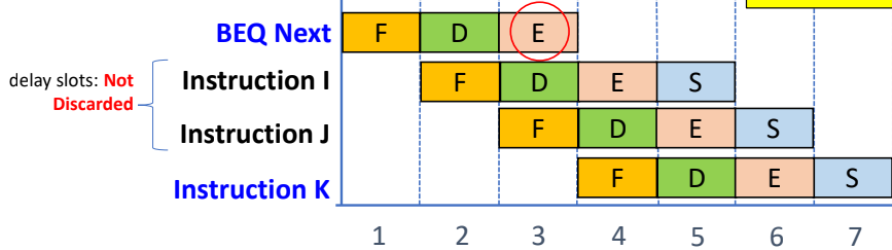
\includegraphics[width=0.3\textwidth]{images/delayed-branching.png}
        \end{center}
        \item \textbf{Solution 3}: Dynamic branch prediction: Implement branch history table that stores (1) address of B instruct, (2) predicted target address, (3) Prediction result (T/F).
        \begin{itemize}
            \item Processor loads instructions based on the prediction. If predict is correct, continue execution and no wasted cycles. If wrong, flush instructions, wasted cycles and update prediction bit and target address for future use.
        \end{itemize}
        \begin{center}
            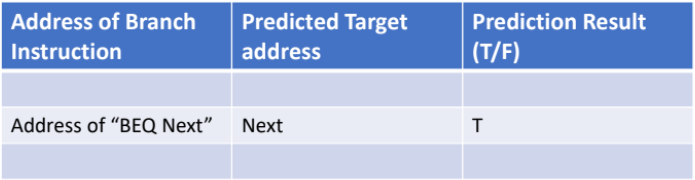
\includegraphics[width=0.3\textwidth]{images/prediction-branch.png}
        \end{center}
    \end{itemize}
\end{enumerate}


\end{multicols}

\end{document}
